\documentclass[tikz, border=5mm]{standalone}
\usepackage{quantikz}

\begin{document}

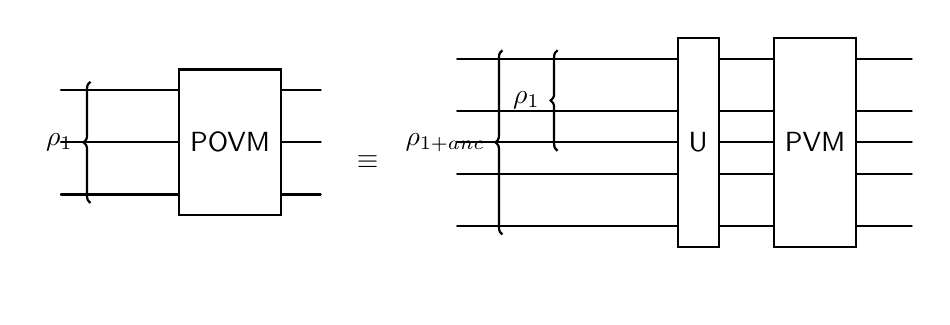
\begin{tikzpicture}
    \node (A) {
        \begin{quantikz}[column sep=0.5cm, row sep=0.4cm]
            & \lstick[3]{$\rho_{1}$} & \qw & \gate[3]{\textsf{POVM}} & \qw \\
            & & \qw & \qw  & \qw                     \\
            & & \qw & \qw  & \qw                     \\
        \end{quantikz}
    };
    \node[right=0.2cm of A] {$\equiv$};
    \node[right=0.7cm of A] (B) {
        \begin{quantikz}[column sep=0.7cm, row sep=0.4cm]
            & \lstick[5]{$\rho_{1 + anc}$} & \lstick[3]{$\rho_{1}$} & \qw & \gate[5]{\textsf{U}} & \gate[5]{\textsf{PVM}} & \qw \\
            & & & \qw & & \qw & \qw \\
            & & & \qw & & \qw & \qw \\
            & & & \qw & \qw   & \qw & \qw  \\
            & & & \qw & \qw   & \qw & \qw  \\
        \end{quantikz}
    };
\end{tikzpicture}

\end{document}